%%%%%%%%%%%%%%%%%%%%
%
% $Autor: Wings $
% $Datum: 2020-02-24 14:29:03Z $
% Projekt: $
% $Version: 1791 $
%
%
%%%%%%%%%%%%%%%%%%%


\chapter{TensorFlow Lite}


\section{Was ist TensorFlow Lite?}

Oft sollen die trainierten Modelle nicht auf dem PC verwendet werden, auf dem sie trainiert wurden, sondern auf mobilen Geräten wie Mobiltelefonen oder Mikrocontrollern oder anderen eingebetteten Systemen. Dort stehen allerdings begrenzte Rechen- und Speicherkapazitäten zur Verfügung. TensorFlow Lite ist ein ganzes Framework, dass die Konvertierung von Modellen in ein spezielles Format und deren Optimierung bezüglich Größe und Geschwindigkeit erlaubt, sodass die Modelle mit TensorFlow Lite-Interpretern dann auf Mobil-, Embedded- und IoT-Geräten ausgeführt werden  können. \cite{Google.09.10.2020}\cite{Warden:2020}

\Mynote{Aufbau des Kapitels}

Bei TensorFlow Lite handelt es sich um eine \glqq light\grqq{} Version von TensorFlow, die für mobile und eingebettete Geräte entwickelt wurde. 
Es erreicht Inferenz mit niedriger Latenz in einer kleinen Binärgröße - sowohl die TensorFlow Lite-Modelle sind viel kleiner. Allerdings kann man ein Modell nicht direkt mit TensorFlow Lite trainieren, sondern es muss zunächst mit TensorFlo erstellt werden, dann muss man das Modell mit dem TensorFlow Lite-Konverter von einer TensorFlow-Datei in eine TensorFlow Lite-Datei konvertieren.\cite{GoogleCoral:2019}
\Mynote{Einführung von TensorFlow Lite-Interpreter und -Konverter?}
Der Grund ist, dass TensorFlow-Modelle üblicherweise bei den neuronalen Netzen in Gleitkommazahlen mit 32-Bit rechnen. Die Gewichte können dabei sehr kleine Werte nahe Null annehmen. Deshalb können die Modelle nicht ohne weiteres auf Systemen ausgeführt werden, die gar nicht mit langen Gleitkommazahlen rechnen können, sondern etwa nur mit Ganzen Zahl mit  8-Bit. Das ist vor allem bei kleinen KI-Prozessoren der Fall, auf denen auf Grund von Größe und Stromverbrauch nur  wenige Transistoren untergebracht werden können. Deshalb muss das neuronale Netz eine Transformation durchlaufen, \glqq bei der aus langen Gleitkommazahlen mit unterschiedlicher Genauigkeit über den darstellbaren Wertebereich -- Gleitkommazahlen bilden den Zahlenbereich um den Nullpunkt viel feiner ab als sehr große oder kleine Werte -- kurze Ganzzahlen mit gleichbleibender Genauigkeit in einem begrenzten Wertebereich werden \grqq \cite{Heise:2020}. Diese Quantisierung findet bei der Überführung in das TensorFlow Lite-Format statt.
 
\section{Ablauf}
 
Der Prozess für den Einsatz von TensorFlow Lite besteht aus vier Schritten:
 
\begin{enumerate}
  \item Wahl eines Modells:
 
      Es kann ein bestehendes, trainiertes Modell übernommen oder selbst trainiert werden oder ein Modell von Grund auf erstellt und trainiert werden.
  \item Konvertierung des Modells:

        Wenn ein benutzerdefiniertes Modell verwendet wird, das dementsprechend nicht im TensorFlow Lite Format vorliegt, muss es mit dem  TensorFlow Lite-Konverter in das Format überführt werden.
  \item Bereitstellung auf dem Endgerät:
  
        Zur Ausführung des Modells auf dem Gerät steht der TensorFlow Lite-Interpreter mit APIs in vielen Sprachen bereit.

 \item Optimierung des Modells:
 
       Es stehen weitere Tools zur Optimierung zur Verfügung, um Modellgröße und Ausführungsgeschwindigkeit zu verbessern. So kann das Modell quantisiert werden, in dem 32-Bit-Gleitkommazahlen in effizientere 8-Bit-Ganzzahlen konvertiert werden. Mit dem TensorFlow Lite-Konverter werden TensorFlow-Modelle in ein optimiertes FlatBuffer-Format umgewandelt, so dass sie vom TensorFlow Lite-Interpreter verwendet werden können. \cite{GoogleTensorFlowLite:2019}       
\end{enumerate}


Die Abbildung~\ref{Software:Flowchart} veranschaulicht den grundlegenden Prozess zur Erstellung eines Modells, das auf einem Edge-Computer verwendet werden kann. Der größte Teil des Prozesses verwendet Standard-TensorFlow-Tools. 

\begin{figure}[!h]
    \centering
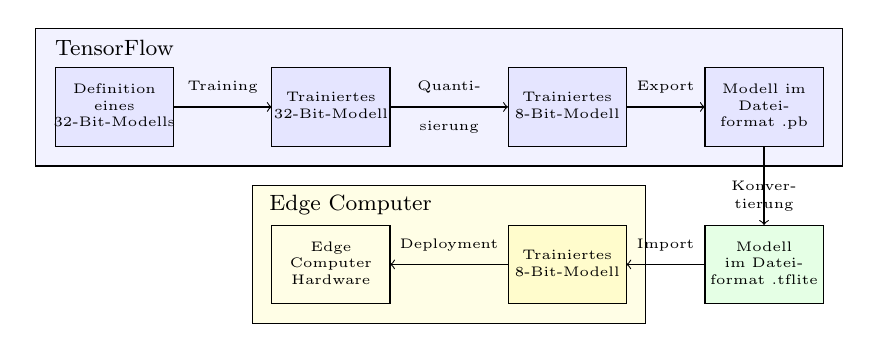
\begin{tikzpicture}
    
  \draw[fill=blue!5] (-0.25,-0.25) -- (10,-0.25) -- (10,1.5) -- (-0.25,1.5) -- cycle;
  \draw[fill=blue!10] (0,0) -- (1.5,0) -- (1.5,1) -- (0,1) -- cycle;
  \node (TF) at (0.75,1.25) {\footnotesize TensorFlow};
  
  \node (T32) at (0.75,0.5) {\tiny \begin{tabular}{c} Definition\\ eines\\ 32-Bit-Modells\\ \end{tabular}};
  
  \node (T32) at (2.125,0.75) {\tiny Training};
  \draw[->] (1.5,0.5) -- (2.75,0.5);
  \draw[fill=blue!10] (2.75,0) -- (4.25,0) -- (4.25,1) -- (2.75,1) -- cycle;
  \node (T32) at (3.5,0.5) {\tiny \begin{tabular}{c}  Trainiertes\\ 32-Bit-Modell\\ \end{tabular}};
  
  \node (T32) at (5.0,0.75) {\tiny Quanti-};
  \node (T32) at (5.0,0.25) {\tiny sierung};
  \draw[->] (4.25,0.5) -- (5.75,0.5);
  \draw[fill=blue!10] (5.75,0) -- (7.25,0) -- (7.25,1) -- (5.75,1) -- cycle;
  \node (T32) at (6.5,0.5) {\tiny \begin{tabular}{c} Trainiertes\\ 8-Bit-Modell\\ \end{tabular}};

  \node (T32) at (7.75,0.75) {\tiny Export};
  \draw[->] (7.25,0.5) -- (8.25,0.5);
  \draw[fill=blue!10] (8.25,0) -- (9.75,0) -- (9.75,1) -- (8.25,1) -- cycle;
  \node (T32) at (9,0.5) {\tiny \begin{tabular}{c} Modell im \\ Datei- \\format .pb\\ \end{tabular}};

  \node (T32) at (9,-0.5) {\tiny Konver- };
  \node (T32) at (9,-0.75) {\tiny tierung};
  \draw[->] (9,0) -- (9,-1);
  \draw[fill=green!10] (8.25,-1) -- (9.75,-1) -- (9.75,-2) -- (8.25,-2) -- cycle;
  \node (T32) at (9,-1.5) {\tiny \begin{tabular}{c} Modell \\im Datei- \\ format .tflite \\ \end{tabular}};

  
  \draw[fill=yellow!10] (2.5,-0.5) -- (7.5,-0.5) -- (7.5,-2.25) -- (2.5,-2.25) -- cycle;
  \node (T32) at (3.75,-0.75) {\footnotesize Edge Computer};
  \node (T32) at (7.75,-1.25) {\tiny Import};
  \draw[<-] (7.25,-1.5) -- (8.25,-1.5);
  \draw[fill=yellow!20] (5.75,-1) -- (7.25,-1) -- (7.25,-2) -- (5.75,-2) -- cycle;

   \node (T32) at (6.5,-1.5) {\tiny \begin{tabular}{c} Trainiertes\\ 8-Bit-Modell\\ \end{tabular}};

  \node (T32) at (5.0,-1.25) {\tiny Deployment};
  \draw[<-] (4.25,-1.5) -- (5.75,-1.5);
  \draw[fill=yellow!10] (2.75,-1) -- (4.25,-1) -- (4.25,-2) -- (2.75,-2) -- cycle;
   \node (T32) at (3.5,-1.5) {\tiny \begin{tabular}{c}  Edge\\ Computer\\ Hardware\\ \end{tabular}};

\end{tikzpicture}  
  
%    \includegraphics[width=0.7\textwidth]{Software/flowchart} 
    
    \caption{Der grundlegende Prozess zur Erstellung eines Modells 
        für einen Edge-Computer\cite{GoogleTensorFlowModel:2019}}\label{Software:Flowchart}
\end{figure}


\section{TensorFlow Lite-Konverter}

Der TensorFlow Lite-Konverter ist ein Tool, das als Python-API verfügbar ist und trainierte TensorFlow-Modelle in das TensorFlow Lite-Format konvertiert. Dazu wird das Keras-Modell in die Form eines FlatBuffers gebracht, ein spezielles platzsparend Dateiformat. Im Allgemeinen wird durch das Konvertieren von Modellen die Dateigröße reduziert und Optimierungen eingeführt, ohne die Genauigkeit zu beeinträchtigen. Der TensorFlow Lite-Konverter bietet weiterhin Optionen, mit denen die Dateigröße weiter reduziert und die Ausführungsgeschwindigkeit erhöht werden kann, was mit mit einigen Kompromissen bezüglich der Genauigkeit einher geht. \cite{Google.09.10.2020}\cite{Warden:2020}

Eine Möglichkeit zur Optimierung ist Quantisierung. Während die Gewichte der Modelle üblicherweise als 32-Bit-Fließkommazahlen gespeichert werden, können sie mit einem nur minimalen Verlust an Genauigkeit des Modells in 8-Bit-Ganzzahlen überführt werden. Das spart Speicherplatz und erlaubt zudem eine schnellere Berechnung, da eine \ac{cpu} mit Ganzzahlen effizienter arbeitet. \cite{Warden:2020}

\section{TensorFlow Lite-Interpreter}

Der TensorFlow Lite-Interpreter ist eine Bibliothek, die ein entsprechend konvertiertes TensorFlow-Lite-Modell unter Verwendung der effizientesten Operationen für das gegebene Gerät ausführt, indem sie die im Modell definierten Operationen auf die Eingabe anwendet und Zugriff auf die Ausgabe bietet. Er funktioniert plattformübergreifend und bietet eine einfache API zum Ausführen von TensorFlow Lite-Modellen aus Java, Swift, Objective-C, C ++ und Python.\cite{Google.09.10.2020}\cite{Warden:2020}

Um die Hardwarebeschleunigung auf verschiedenen Geräten zu nutzen, kann der TensorFlow Lite-Interpreter mit \glqq Delegates\grqq konfiguriert werden. Diese nutzen Gerätebeschleuniger wie eine \ac{gpu} oder einen digitalen Signalprozessor (DSP). \cite{Google.09.10.2020}

